\documentclass[aspectratio=169, 14pt]{beamer}
\usepackage[utf8]{inputenc}
\usepackage[english]{babel}
\usepackage{tipa}
\usepackage{graphicx}
\usepackage{transparent}
\usepackage{xeCJK}
\usepackage[ruled, lined, linesnumbered, commentsnumbered]{algorithm2e}
\usepackage{tikz}
\usetikzlibrary{calc,shadows.blur}
\usetikzlibrary{matrix,backgrounds}
\usepackage{pgfplots}
\pgfplotsset{compat=1.13}
\usepackage{minted}
\usepackage{csquotes}
\usepackage{outlines}
\usepackage{booktabs}
\usepackage{hyperref}
\hypersetup{
    colorlinks=true,
    linkcolor=blue,
    filecolor=magenta,      
    urlcolor=cyan,
    }
\urlstyle{same}
\usetheme{metropolis}
\metroset{block=fill}
\usecolortheme{default}
\definecolor{darkmidnightblue}{rgb}{0.0, 0.2, 0.4}
\definecolor{LightGray}{gray}{0.9}


%------------------------------------------------------------
%This block of code defines the information to appear in the
%Title page
\title[Data Structures] %optional
{Data Structures}

\subtitle{Algorithm Analysis and TDD}

\author[CHEN Zhongpu] % (optional)
{CHEN Zhongpu}

\institute[] % (optional)
{
  School of Computing and Artificial Intelligence \\
  \href{mailto:zpchen@swufe.edu.cn}{zpchen@swufe.edu.cn}
}

\date[] % (optional)
{SWUFE, Fall 2022}

%End of title page configuration block
%------------------------------------------------------------


%------------------------------------------------------------
%The next block of commands puts the table of contents at the 
%beginning of each section and highlights the current section:

% \AtBeginSection[]
% {
%   \begin{frame}
%     \frametitle{Table of Contents}
%     \tableofcontents[currentsection]
%   \end{frame}
% }
%------------------------------------------------------------


\begin{document}

%The next statement creates the title page.
\frame{\titlepage}

%---------------------------------------------------------
%This block of code is for the table of contents after
%the title page
% \begin{frame}
% \frametitle{Table of Contents}
% \tableofcontents
% \end{frame}
%--------------------------------------------------------
\begin{frame}
    \frametitle{A Small Quiz}
    \begin{enumerate}
        \item<1->  Can we add the 11th element onto an \alert{ArrayList} in Java whose size is 10?
        \item<2->  How to access the last element of a 
        \alert{list} in Python?
        \item<3->  Given \texttt{bag = \{1, 1, 2, 2, 3\}}, what is the size of it?
    \end{enumerate}
\end{frame}

{
    % \usebackgroundtemplate{\transparent{0.3}{\begin{picture}
    %     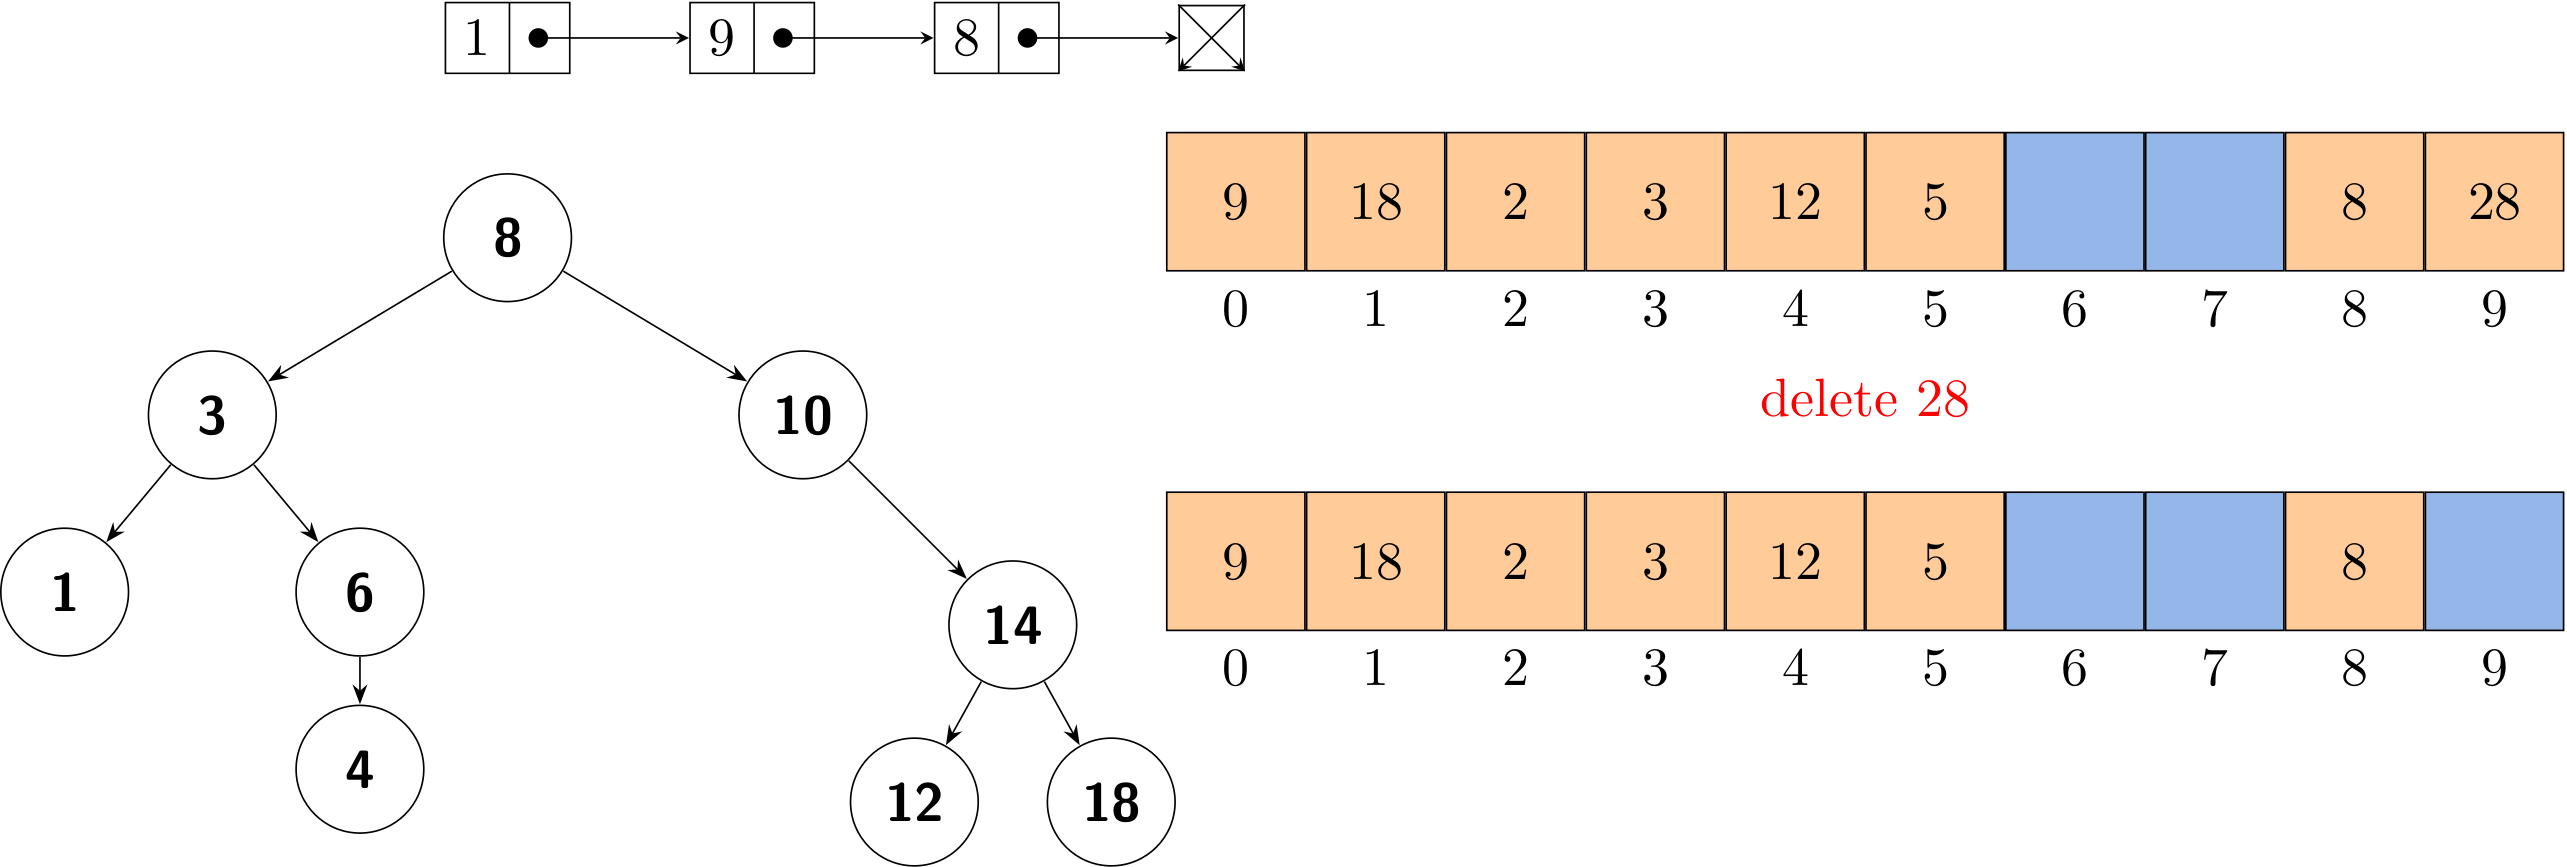
\includegraphics[height=0.7\paperheight]{cover}
    % \end{picture}    
    % }}
\usebackgroundtemplate{
  \tikz[overlay,remember picture] 
  \node[opacity=0.3, at=(current page.south east),anchor=south east, yshift=2cm,xshift=4cm] {
    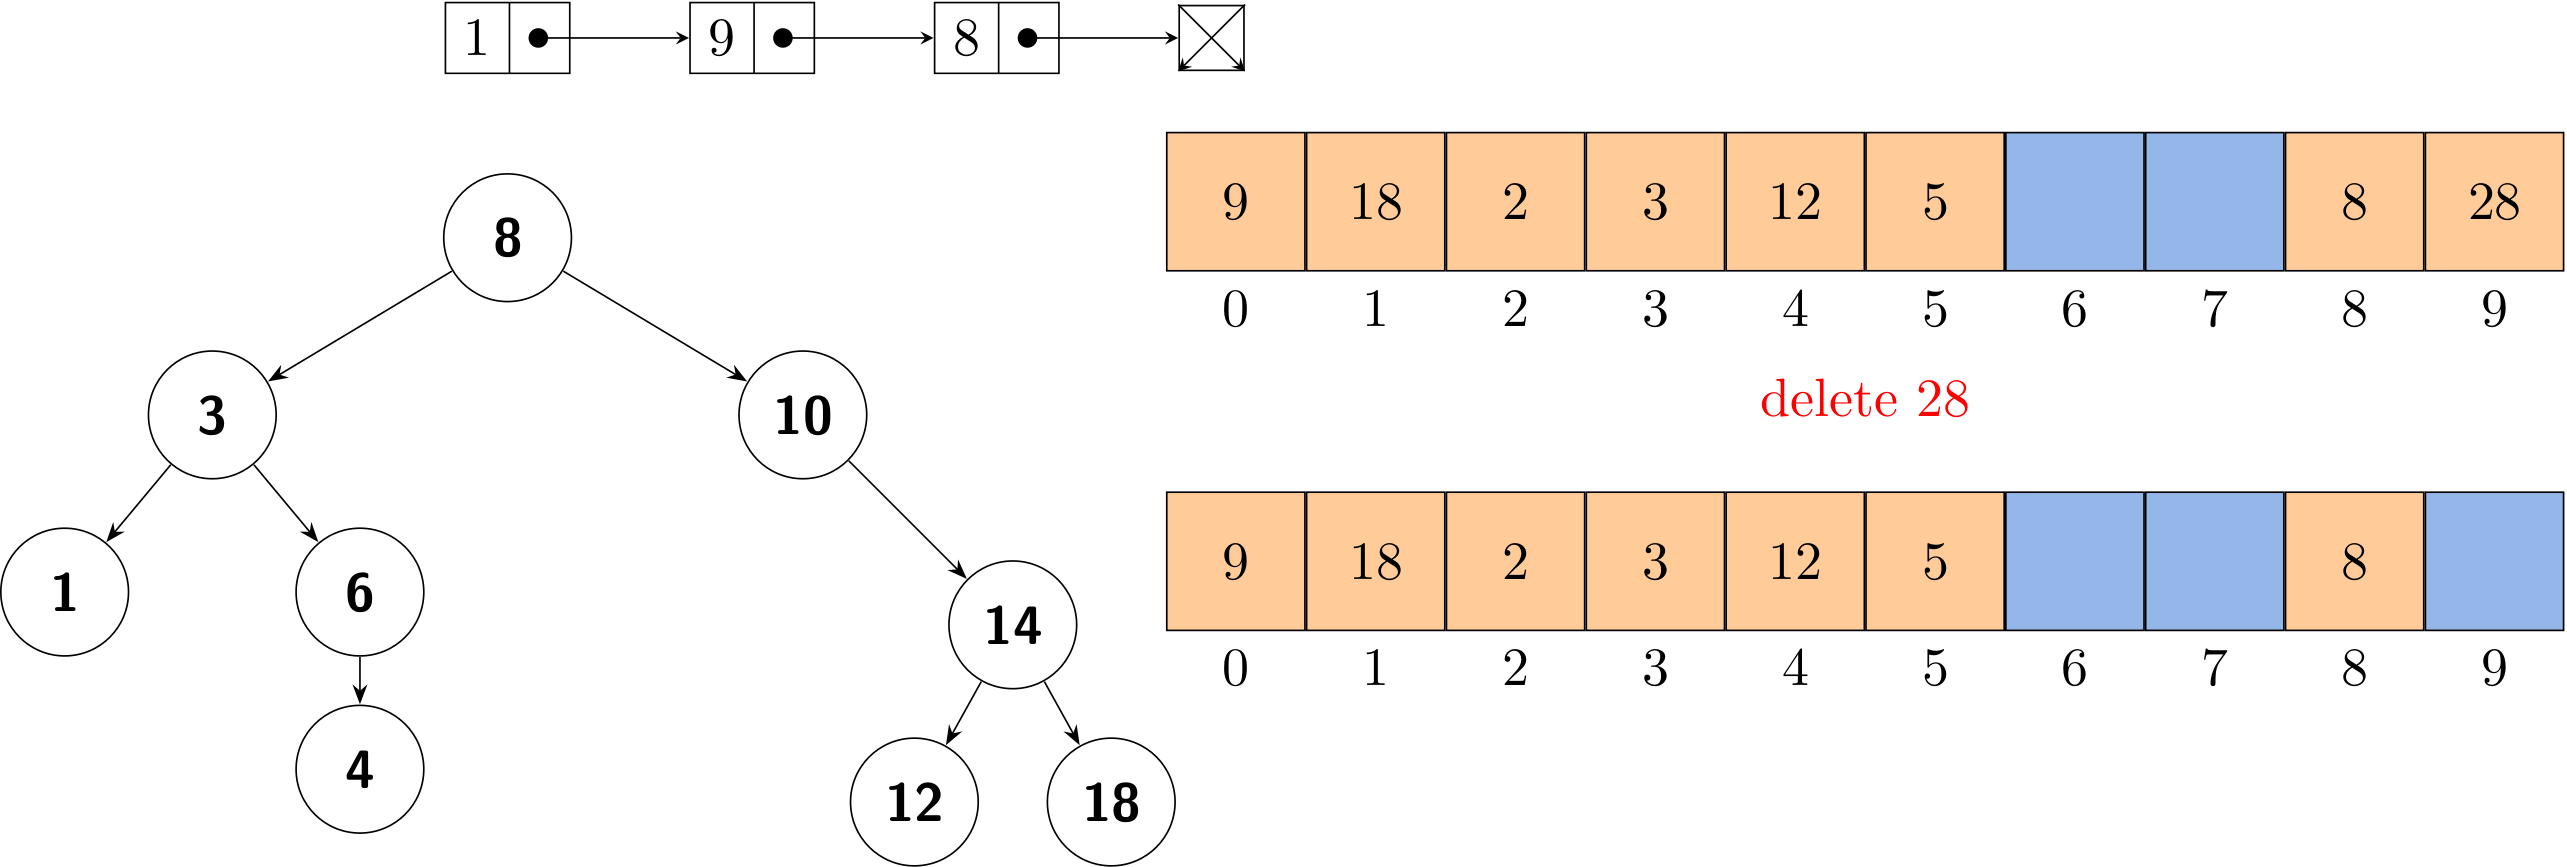
\includegraphics[height=0.6\paperheight]{cover}};
}
    \begin{frame}
        \section{\textcolor{darkmidnightblue}{Algorithm Analysis}}
    \end{frame}
}
\begin{frame}[fragile]
    \frametitle{How Fast Is A Program?}
    \begin{block}{Fact 2}
        \textbf{Different data structures have varying (time) \alert{efficiencies}.}
    \end{block} 
A straightforward way is to measure the elapsing time.
\begin{minted}[bgcolor=LightGray]{java}
long start = System.currentTimeMillis();
// your program runs
long end = System.currentTimeMillis();
long elapse = end - start;    
\end{minted}
\end{frame}

\begin{frame}[fragile]
    \frametitle{How Fast Is A Program?}
    \begin{block}{Fact 2}
        \textbf{Different data structures have varying (time) \alert{efficiencies}.}
    \end{block} 
A straightforward way is to measure the elapsing time.
\begin{minted}[bgcolor=LightGray]{python}
start = int(round(time.time() * 1000))
# your program runs
end = int(round(time.time() * 1000))
elapse = end - start    
\end{minted}
\end{frame}

\begin{frame}[fragile]
\texttt{1, 1, 2, 3, 5, 8, 13, ...}
    \begin{minted}[bgcolor=LightGray]{python}
def fibonacci(n):
    if n == 0:
        return 0
    elif n == 1 or n == 2:
        return 1
    else:
        return fibonacci(n - 1) + fibonacci(n - 2)        
    \end{minted}
Which will cost more time? \texttt{fibonacci(10)}, or \texttt{fibonacci(20)}? 

Intuitively, the time cost grows with the input size (\emph{problem size}).
\end{frame}

\begin{frame}
\begin{block}{Gravity}
    Suppose you were in the year of 1660 by time travel, how could you measure the gravity ($9.8 m/s$)?
\end{block}
\pause
    \begin{itemize}
        \item \textbf{Observe} some feature of the natural world.
        \item \textbf{Hypothesize} a model that is consistent with the observations.
        \item \textbf{Predict} events using the hypothesis.
        \item \textbf{Verify} the predictions by making further observations.
        \item \textbf{Validate} by repeating until the hypothesis and observations agree.
    \end{itemize}

\end{frame}

\begin{frame}[fragile]

Still, you will find yourself asking the more detailed question: \textbf{How long will my program take, as a function of the input size?} To help answer this question, we plot the data. 

\begin{minted}[bgcolor=LightGray]{python}
if __name__ == '__main__':
    ns = [20, 21, 22, 23, 24, 25, 26, 27, 28, 29, 30]
    with open('fib_python.txt', 'w') as f:
        for n in ns:
            start = int(round(time.time() * 1000))
            fibonacci(n)
            end = int(round(time.time() * 1000))
            f.write(f'{n}   {end - start}\n')
\end{minted}

\end{frame}

\begin{frame}
    \frametitle{Plot}
\begin{columns}
    \column{0.6\textwidth}
    \begin{center}
        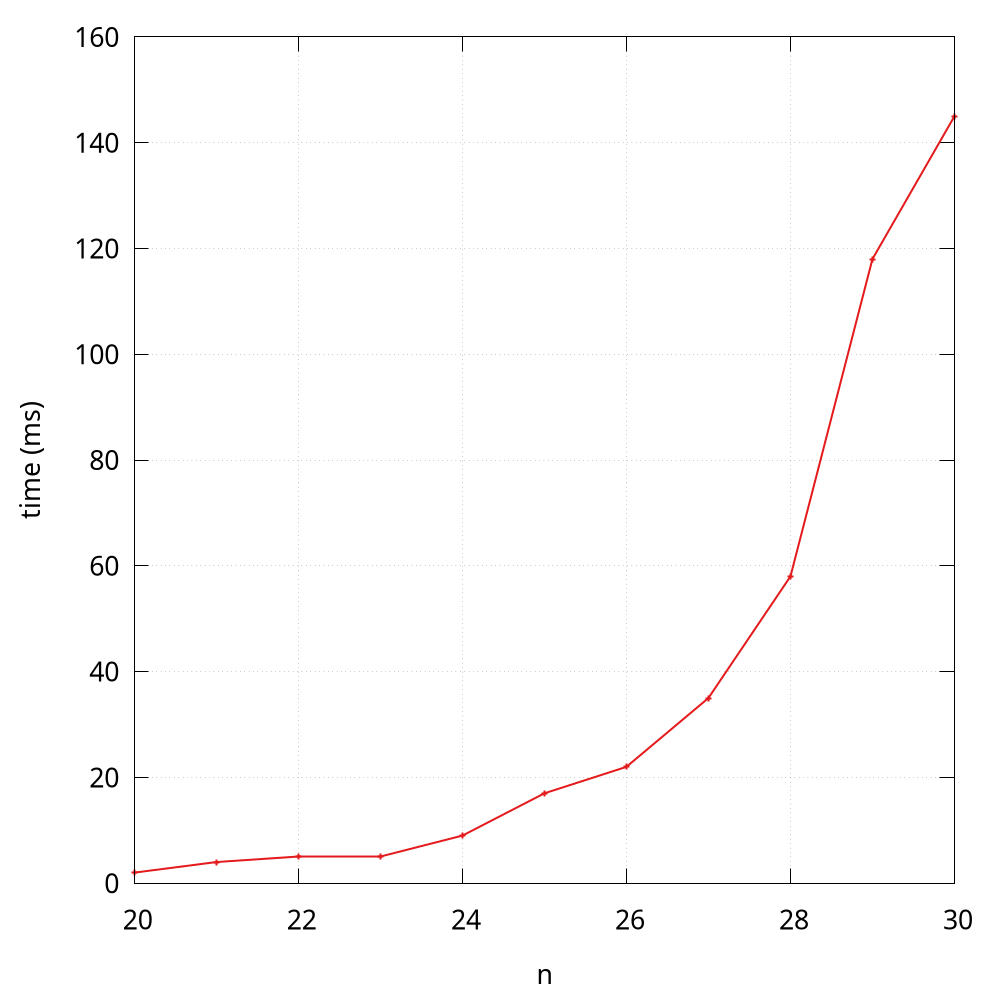
\includegraphics[height=.8\paperheight]{week2/fib_python}    
    \end{center}
    \column{0.4\textwidth}
    Popular visualization tools:  \texttt{gnuplot}, \texttt{ggplot2} in R, \texttt{Matplotlib} in Python, and \texttt{Plotly Express} in Python.

\end{columns}
\end{frame}

\begin{frame}
    \frametitle{Mathematical Models}
\(g = \frac{GM}{r^2}\), \(t(n) = a2^{n}\)

\begin{exampleblock}{Knuth's insight}
The total running time of a program is determined by two primary factors:
\begin{enumerate}
    \item The cost of executing each statement
    \item The frequency of execution of each statement
\end{enumerate}
\end{exampleblock}

\end{frame}

\begin{frame}[fragile]
What is the frequency of the inner \alert{print} statement?
\begin{minted}[bgcolor=LightGray]{python}
def foo(n):
    for i in range(n):
        print(i)
\end{minted}
What is the frequency of the inner \emph{assignment} statement?
\begin{minted}[bgcolor=LightGray]{python}
def cubic_sum(n):
    s = 0
    for i in range(1, n+1):
        s += i * i * i
    return s
\end{minted}
\end{frame}

\begin{frame}[fragile]
    What is the frequency of the inner \alert{if} statement?
    \begin{minted}[bgcolor=LightGray]{python}
    def two_sum(self, nums, target):
        for i, v in enumerate(nums):
            for j in range(i + 1, len(nums)):
                if v + nums[j] == target:
                    return [i, j]
        return []
    \end{minted}
    

\end{frame}

\begin{frame}
    \begin{block}{Revisit}
        Suppose there are $10^6$ books in an array. To find a book titled \emph{``Gone with the wind"}, how many times is the comparison performed?
        \begin{enumerate}
            \item On the \textbf{best} case: 1 
            \item On the \textbf{worst} case: $10^6$
            \item On the \textbf{average} case $10^6/2$
        \end{enumerate}
    \end{block}
\end{frame}

\begin{frame}[fragile]
    \frametitle{Approximate Running Time}

    \begin{columns}
        \column{0.4\textwidth}
        Compare $\frac{n^2 - n}{2}$ and $\frac{n^2}{2}$.
        
        We can say \alert{$\frac{n^2}{2} \sim \frac{n^2 - n}{2}$}, because $\frac{n^2}{2}$ is similar to $\frac{n^2 - n}{2}$ as $n$ grows. 
        \column{0.6\textwidth}
    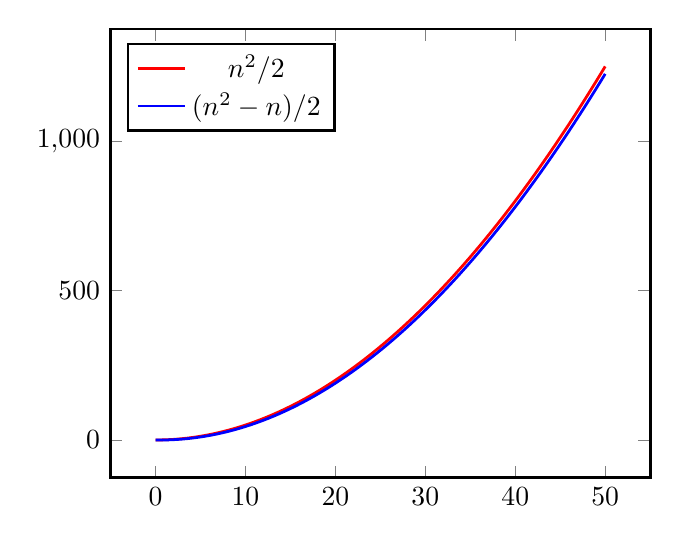
\begin{tikzpicture}
        \begin{axis}[legend pos=north west,line width=1pt]
        \addplot[color=red, domain=0:50,samples=100]{x*x/2};
        \addlegendentry{\(n^2/2\)}
        \addplot[color=blue, domain=0:50,samples=100]{(x*x - x)/2};
        \addlegendentry{\((n^2-n)/2\)}
        \end{axis}
    \end{tikzpicture}
    \end{columns}
\end{frame}

\begin{frame}[fragile]
\begin{exampleblock}{Tilde Approximation}
    We write $\sim f(n)$ to represent any function that, when divided by $f(n)$, approaches 1 as $n$ grows, and we write $g(n) \sim f(n)$ to indicate that $g(n)/f(n)$ approaches 1 as $n$ grows.
\end{exampleblock}    
\pause
Given $g(n)\sim af(n)$, we can say the \textbf{order of growth} of $g(n)$ is $f(n)$ because the constant $a$ won't change the growth tendency.
\end{frame}

\begin{frame}
\begin{quote}
    The \alert{order of growth} of an algorithm is an approximation of the time required to run a computer program as the input size increases.
\end{quote}
    

\end{frame}

\begin{frame}[fragile]
    \frametitle{Approximation Examples}

    \begin{table}
        \caption{Some typical approximations}
        \begin{tabular}{lll}
          \toprule
          Function & Approximation & Order of growth \\
          \midrule
          $n^3/6 - n^2/2 + n/3$ & $n^3/6$ & $n^3$ \\
          $n^2/2 - n/2$ & $n^2/2$ & $n^2$ \\
          $\lg{n} + 1$ & $lg{n}$ & $lg{n}$ \\
          $3$ & $3$ & $1$ \\
          \bottomrule
        \end{tabular}
    \end{table}
\end{frame}
\begin{frame}
    \frametitle{Big O Notation}

    \begin{columns}
        \column{0.4\textwidth} 
        The order of growth \textbf{in the worst case} can be also described by the \alert{big O} notation in terms of \textbf{time complexity}. 
        \column{0.59\textwidth}  
        \begin{table}
            \caption{Common time complexity descriptions}
            \begin{tabular}{ll}
              \toprule
              Description & Time complexity \\
              \midrule
              constant	& $O(1)$ \\
        logarithmic	& $O(log{n})$ \\
        linear	& $O(n)$ \\
        linearithmic	& $O(nlog{n})$ \\
        quadratic	& $O(n^2)$ \\
        cubic	& $O(n^3)$ \\
        exponential	& $O(2^n)$ \\
              \bottomrule
            \end{tabular}
        \end{table}
    \end{columns}
\end{frame}

\begin{frame}
Suppose $f(x)$ and $g(x)$ are two functions defined on some subset of the real numbers. We write 

\[f(x) = O(g(x))\]

if and only if there exists constants $N$ and $C$ such that

\[|f(x)| \leq Cg(x), \forall x > N\]
    

Intuitively, this means that $f$ does not grow faster than $g$ ($g$ is the \alert{upper bound} of $f$).

\end{frame}

\begin{frame}[fragile]
    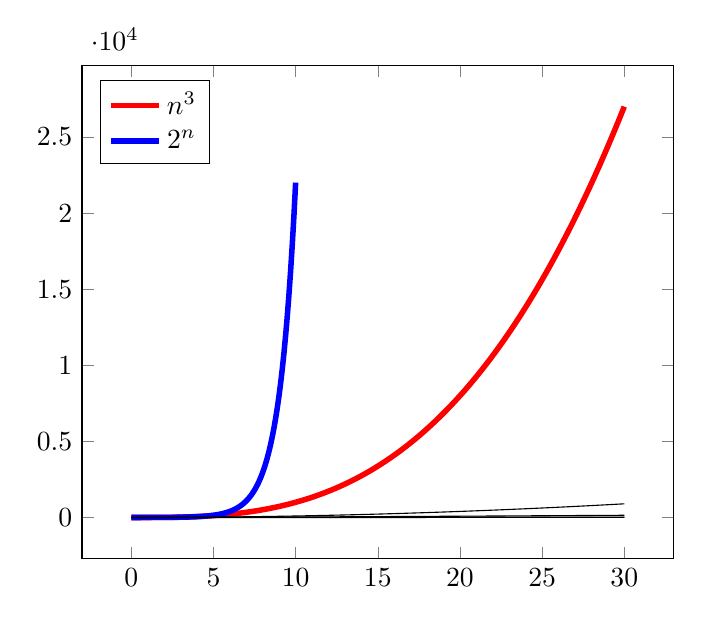
\begin{tikzpicture}
        \begin{axis}[legend pos=north west, width=.75\textwidth]
        \addplot[color=red, domain=0:30,samples=100, line width=2pt]{x^3};
        \addlegendentry{\(n^3\)}
        \addplot[color=blue, domain=0:10, samples=100, line width=2pt]{exp(x)};
        \addlegendentry{\(2^n\)}
        \addplot[domain=0:30,samples=100]{1}; 
        \addplot[domain=0:30,samples=100]{log2(x)};  
        \addplot[domain=0:30,samples=100]{x};
        \addplot[domain=0:30,samples=100]{x*log2(x)};
        \addplot[domain=0:30,samples=100]{x^2};
        \end{axis}
    \end{tikzpicture} 
\end{frame}

\begin{frame}[fragile]
    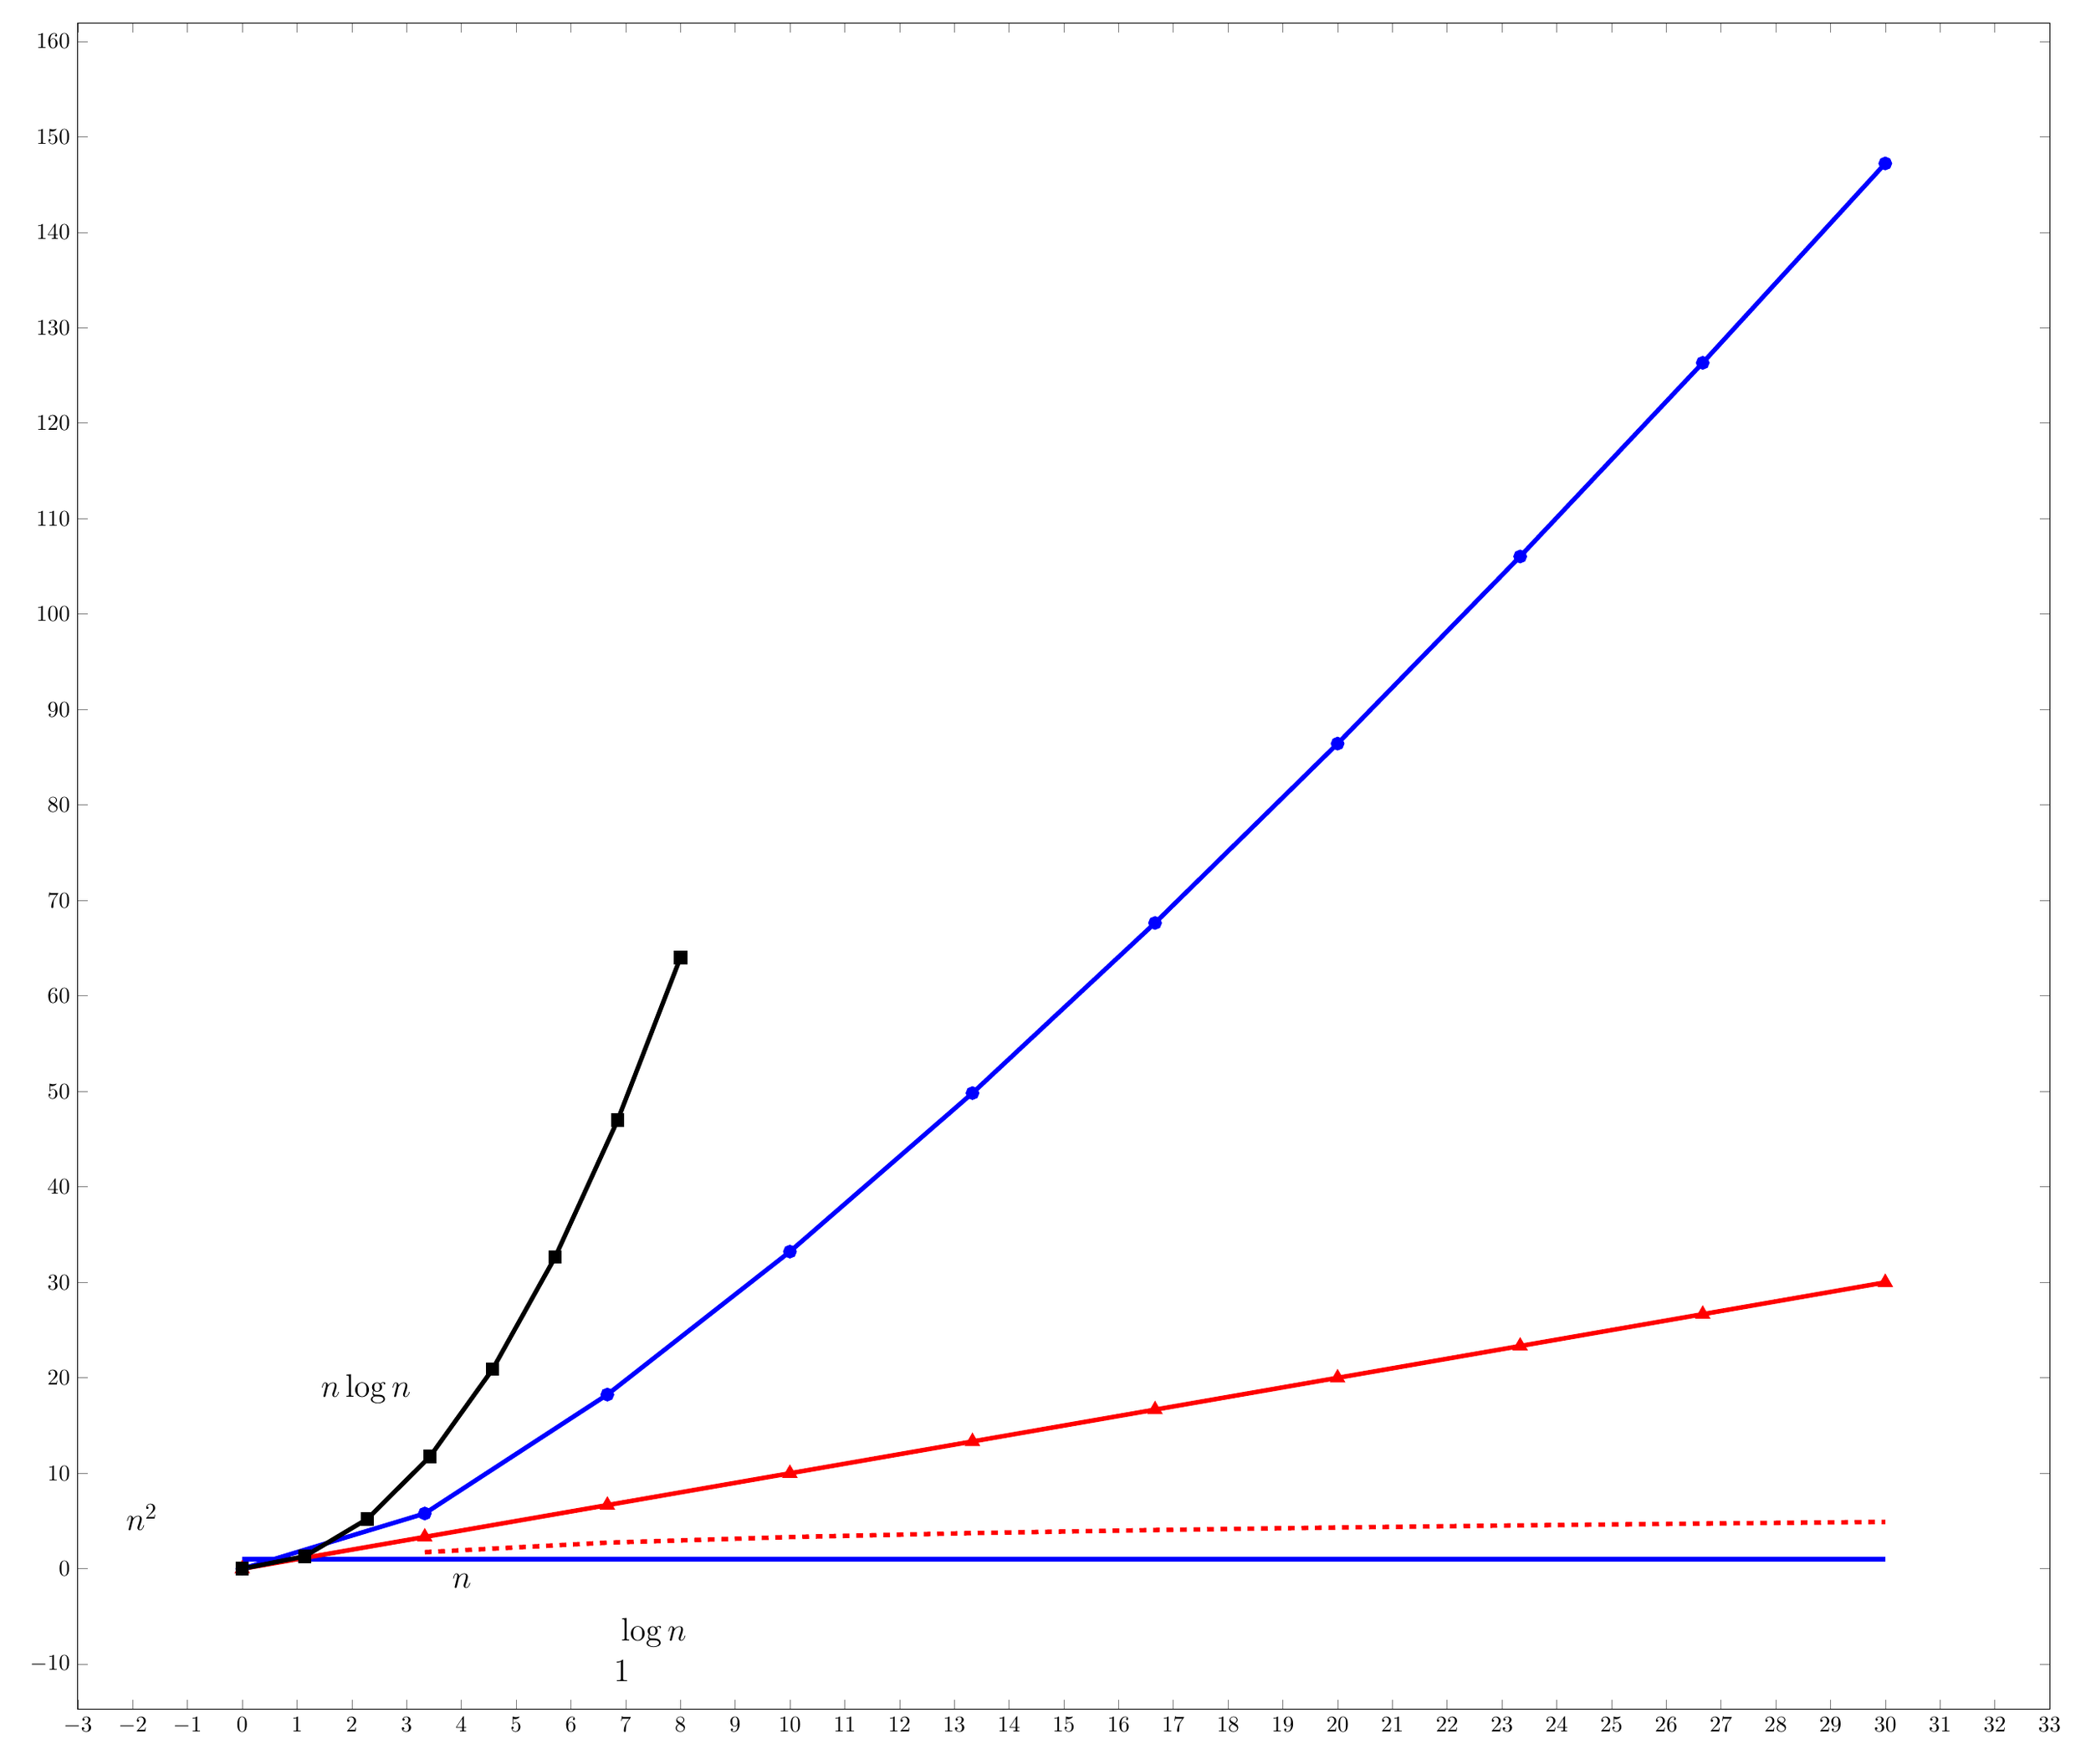
\begin{tikzpicture}
        \begin{axis}[legend pos=north west, height=1\paperheight]
        \addplot[blue, domain=0:30,samples=100, line width=2pt]{1}; 
        \addplot[domain=0:30,samples=10, dashed, red, line width=2pt]{log2(x)};  
        \addplot[red, mark=triangle*, domain=0:30,samples=10, line width=2pt]{x};
        \addplot[blue, mark=*,domain=0:30,samples=10, line width=2pt]{x*log2(x)};
        \addplot[mark=square*, domain=0:8,samples=8, line width=2pt]{x^2};
        \end{axis}
        \node at (1, 3) {\Large $n^2$};
        \node at (4.5, 5) {\Large $n\log{n}$}; 
        \node at (6, 2) {\Large $n$};
        \node at (9, 1.2) {\Large $\log{n}$}; 
        \node at (8.5, 0.6) {\Large $1$}; 
    \end{tikzpicture} 

\end{frame}

\begin{frame}[fragile]
    What is the time complexity of \texttt{foo()} and \texttt{two\_sum()}, respectively? 
    \begin{minted}[bgcolor=LightGray]{python}
    def foo(n):
        for i in range(n):
            print(i)
    \end{minted}

    \begin{minted}[bgcolor=LightGray]{python}
    def two_sum(self, nums, target):
        for i, v in enumerate(nums):
            for j in range(i + 1, len(nums)):
                if v + nums[j] == target:
                    return [i, j]
        return []
    \end{minted}
\end{frame}

\begin{frame}[fragile]
    \frametitle{Exercise}
\begin{minted}[bgcolor=LightGray]{python}
def selection_sort(a):
    n = len(a)
    for i in range(n):
        m_idx = i
        for j in range(i + 1, n):
            if a[j] < a[m_idx]:
                m_idx = j
        a[i], a[m_idx] = a[m_idx], a[i]    
\end{minted}
\end{frame}

\begin{frame}[fragile]
\begin{minted}[bgcolor=LightGray]{python}
def search(a, target):
    high = len(a) - 1
    low = 0
    while high >= low:
        mid = low + (high - low) // 2
        if a[mid] == target:
            return mid
        elif a[mid] > target:
            high = mid - 1
        else:
            low = mid + 1
    return -1  
\end{minted}    

\end{frame}

\begin{frame}
    \frametitle{Revisit Fibonacci}
\begin{columns}
    \column{0.6\textwidth}
    \begin{center}
        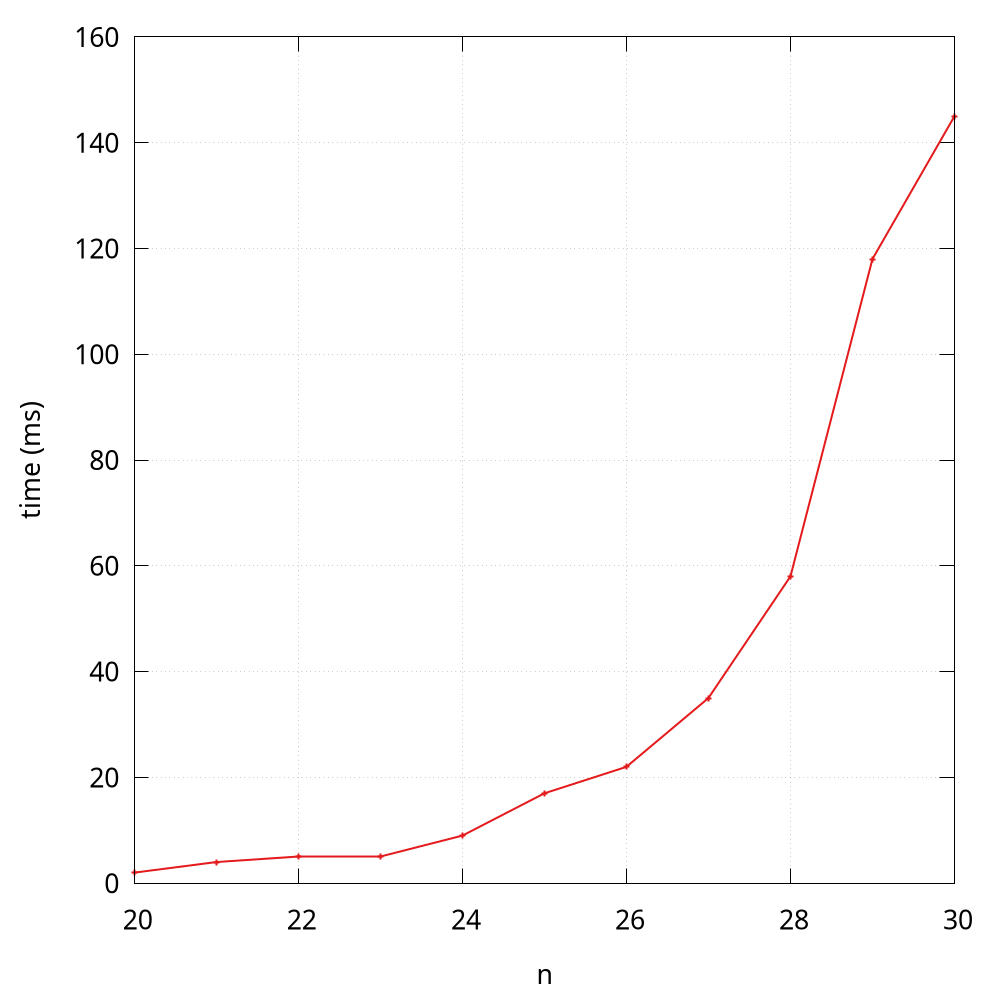
\includegraphics[height=.8\paperheight]{week2/fib_python}    
    \end{center}
    \column{0.4\textwidth}
The time complexity of fibonacci is $O(2^n)$.

\end{columns}

\end{frame}

\begin{frame}
    \frametitle{A Final Note}
\begin{alertblock}{Note}
    A comprehensive about algorithm analysis is out of the scope of this course. You should at least understand:
    
    \begin{itemize}
        \item How to use big O notation to express how complex an algorithm is;
        \item How to use plots to help you evaluate an algorithm.
    \end{itemize}
\end{alertblock}
\end{frame}

\section{\textcolor{darkmidnightblue}{Test-driven Development}}
\begin{frame}[fragile]
    \frametitle{TDD}
    \begin{exampleblock}{Question}
    How can you make sure that a program is correct?
    \end{exampleblock}
    \begin{minted}[bgcolor=LightGray]{java}
public int add(int a, int b) {
    return a + b;
} 
    \end{minted} 
\end{frame}

\begin{frame}[fragile]
    \begin{minted}[bgcolor=LightGray, baselinestretch=0.95]{java}
public int search(List<Integer> list, int target) {
    int high = list.size() - 1;
    int low = 0;
    while (high >= low) {
        int mid = low + (high - low) / 2;
        if (list.get(mid) == target) {
            return mid;
        } else if (list.get(mid) > target) {
            high = mid - 1;
        } else {
            low = mid + 1;
        }
    }
    return -1;
}
    \end{minted} 
\end{frame}

\begin{frame}[fragile]
    \frametitle{Assert}
    Many beginners would simply print the outputs, but it can be tedious to figure out where bugs are.

\pause
An \alert{assertion} allows testing the correctness of any assumptions that have been made in the program, and once \texttt{assert} fails, the program will crash. 

\begin{minted}[bgcolor=LightGray]{java}
Fibonacci f = new Fibonacci();
assert f.fibonacci(5) == 5;
\end{minted}

\begin{minted}[bgcolor=LightGray, baselinestretch=0.95]{python}
assert fibonacci(5) == 5
\end{minted}

\end{frame}

\begin{frame}[fragile=singleslide]
    Note that \texttt{assert} is enabled in Python by default. To disable it, you can call Python with the \alert{-O} flag.

    \begin{verbatim}
        python3 -O <your program>
    \end{verbatim}

    Also note that \texttt{assert} is disabled in Java by default. To enable is, you can run the program with the \alert{-ea} flag.

    \begin{verbatim}
        java -ea <your program>
    \end{verbatim} 
\end{frame}

\begin{frame}[fragile]
The main usage of \alert{assert} is: \textbf{it should (not) meet some conditions}.

For example, \texttt{fibonacci(-2)} does not make sense:

\begin{minted}[bgcolor=LightGray]{python}
def fibonacci(n):
    assert n > 0
    if n == 0:
        return 0
    elif n == 1 or n == 2:
        return 1
    else:
        return fibonacci(n - 1) + fibonacci(n - 2) 
\end{minted}  

\end{frame}

\begin{frame}
    \frametitle{Unit Test}
\begin{quote}
    For modern software engineering, the test driven development (TDD) is widely adopted, and \alert{unit tests} serve as an essential component in TDD. 
\end{quote}

A unit test should:
\begin{itemize}
    \item test one method
    \item provide some specific arguments to that method
    \item test that the result is as expected
\end{itemize}
\end{frame}

\begin{frame}[fragile]

    \begin{minted}[bgcolor=LightGray]{java}
public class Add {
    public int add(int a, int b) {
        return a + b;
    }
}
    \end{minted}  
In Java, the most popular unit test framework is \href{https://junit.org/junit5/}{JUnit 5}.

\begin{minted}[bgcolor=LightGray]{java}
@Test
void add() {
    Add a = new Add();
    assertEquals(a.add(1, 2), 3);
}    
\end{minted}

\end{frame}

\begin{frame}[fragile]
In Python, the \href{https://docs.python.org/3/library/unittest.html}{unittest} module, inspired by JUnit, has a similar flavor as major unit testing frameworks in other languages.
\begin{minted}[bgcolor=LightGray]{python}
class Test(TestCase):
    def test_add(self):
        self.assertEqual(add(2, 1), 3)

    def test_add_negatives(self):
        self.assertEqual(add(-2, -2), -4)    
\end{minted}

\end{frame}


\begin{frame}
    \begin{center}
        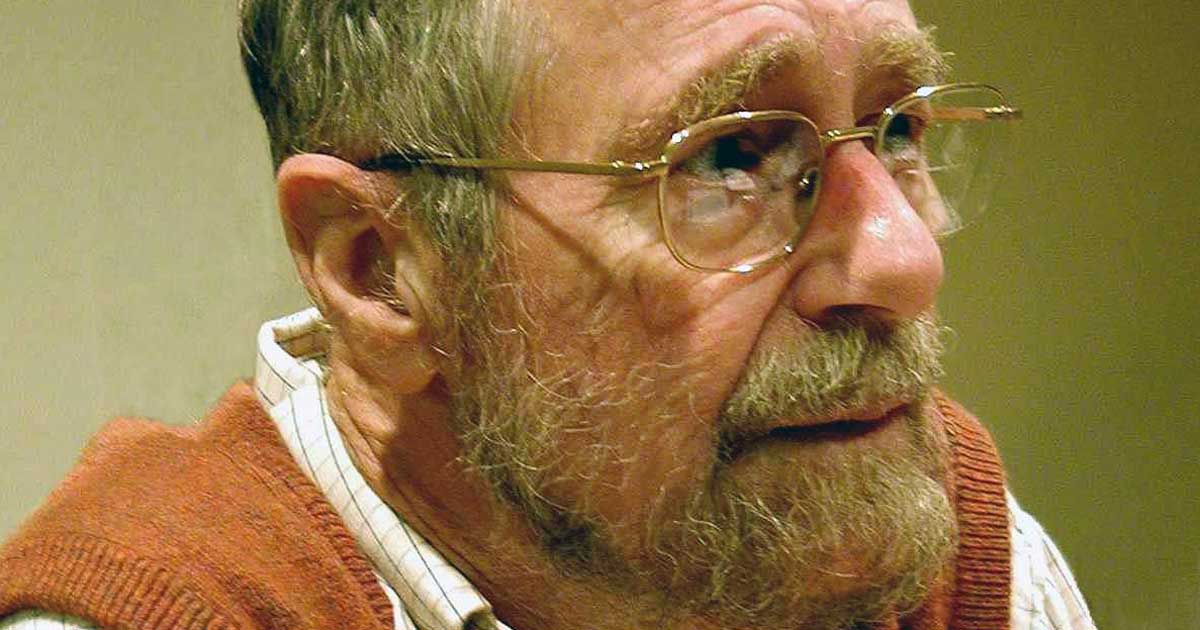
\includegraphics[height=.4\paperheight]{week2/dijkstra}
    \end{center}

   \begin{quote}
    Program testing can be a very effective way to show the presence of bugs, but it is hopelessly inadequate for showing their absence.
    \begin{flushright}
        --- Edsger W. Dijkstra
    \end{flushright}
   \end{quote} 

\end{frame}

\begin{frame}
    \section{\textcolor{darkmidnightblue}{Conclusion}}

    \begin{enumerate}
        \item Big O notation
        \item Evaluation through visualization
        \item Unit test
    \end{enumerate}
\end{frame}

\begin{frame}
    \frametitle{Homework 1}
All exercises can be found on the online book \href{https://chenzhongpu.github.io/data-structure-swufe/}{Hands On Data Structures}.    

\begin{enumerate}
    \item Ex4, Chapter 1 (5 marks)
    \item Ex5, Chapter 1 (5 marks)
\end{enumerate}
\begin{tikzpicture}
    \node[fill=yellow,blur shadow={shadow xshift=-0.5ex},
    text width=25em,anchor=south west,rounded corners]
    {Please submit your homework before the deadline through \textbf{FeiShu Document}. Please follow the naming rule: \alert{HW<n>\_YourName\_StudentNum} (e.g., HW1\_李大锤\_2020123).
    };
\end{tikzpicture} 
\end{frame}

\end{document}